\begin{figure}[h]
  \centering
  %Define block styles
  \tikzstyle{decision} = [diamond, draw, fill=blue!20, 
  text width=4.5em, text badly centered, node distance=3cm, inner sep=0pt]
  \tikzstyle{block} = [rectangle, draw, fill=blue!20, text width=12em, text
  centered, rounded corners, minimum height=3em]
  \tikzstyle{line} = [draw, -latex']
  \tikzstyle{cloud} = [fill=none, node distance=3cm, minimum
  height=2em]
  
    
  \begin{tikzpicture}[node distance = 2cm, auto]
    % Place nodes
    \node[cloud] (theory) {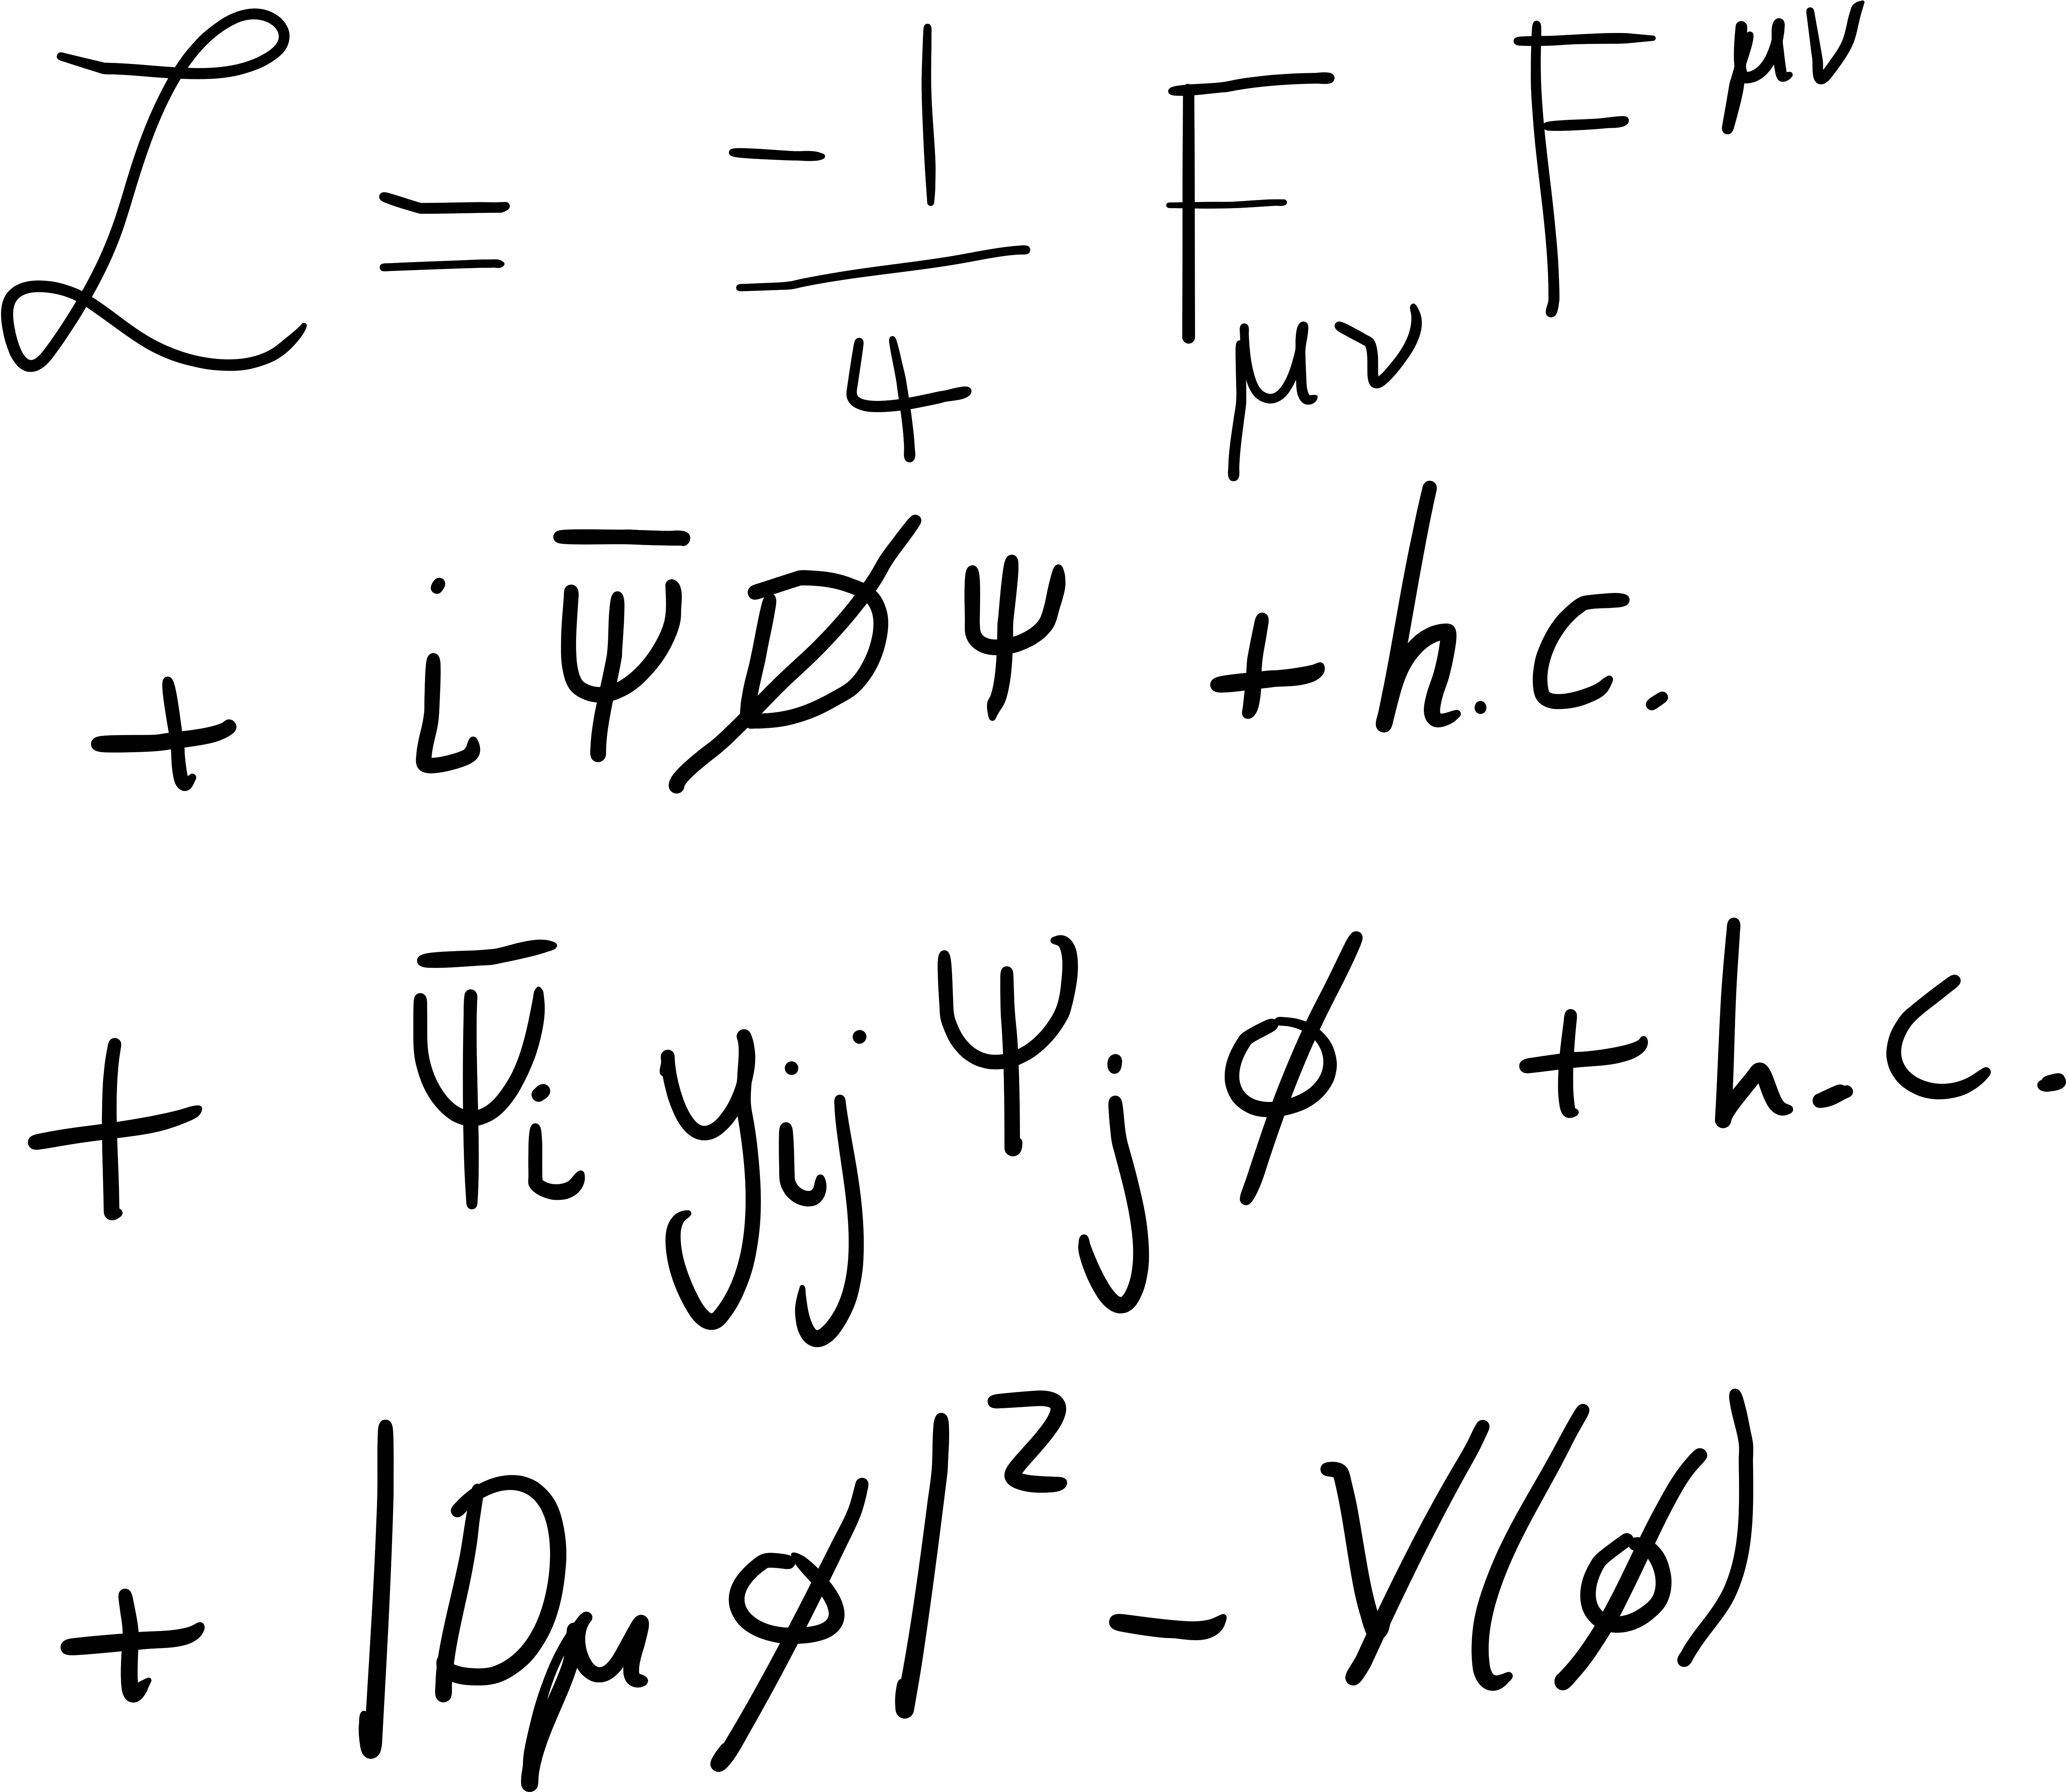
\includegraphics[width=.25\textwidth]{hand_written_lagrangian-1
      }};
    
    \node [cloud, right=1.5cm of theory] (detector)  {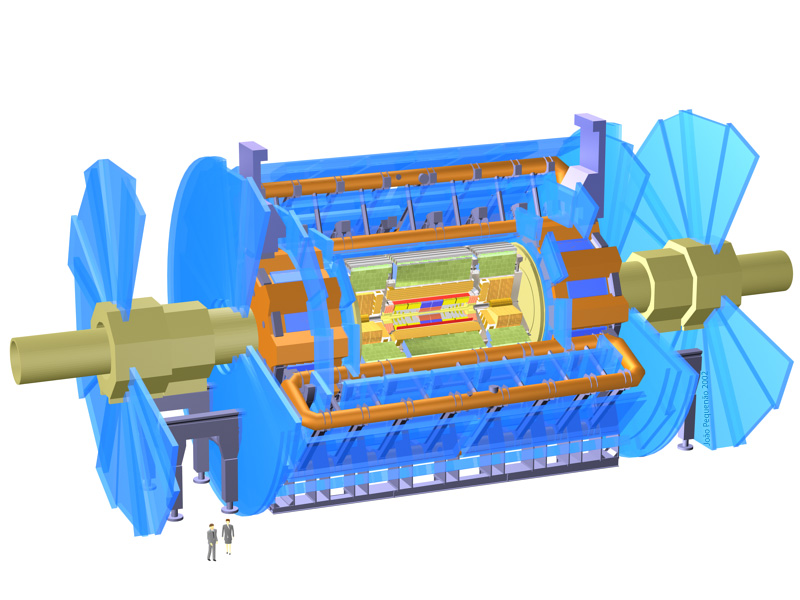
\includegraphics[width=.25\textwidth]{atlas_big}};

    
    % Draw edges 
    \path [line] (theory) -- (detector);
    
  \end{tikzpicture}
  \caption{A flow chart showing the roadmap of the VHbb analysis and of this thesis.}
  \label{fig:cxaod-flow}
\end{figure}
